\documentclass{article}

\usepackage{fancyhdr} % Required for custom headers
\usepackage{lastpage} % Required to determine the last page for the footer
\usepackage{extramarks} % Required for headers and footers
\usepackage[usenames,dvipsnames]{color} % Required for custom colors
\usepackage{graphicx} % Required to insert images
\usepackage{listings} % Required for insertion of code
\usepackage{courier} % Required for the courier font
\usepackage{lipsum} % Used for inserting dummy 'Lorem ipsum' text into the template
\usepackage{hyperref}
\usepackage{multirow}
\usepackage{tabularx}
\usepackage{longtable}
\usepackage{framed}
\usepackage{listings}
\usepackage{subfigure}
\usepackage{afterpage}
\usepackage{amsmath,amssymb}            
\usepackage{rotating}  
\usepackage{fancyhdr}
\usepackage{graphicx}
\usepackage{amsthm}
\usepackage[scriptsize]{caption} 
\hyphenation{a-gen-tiz-za-zio-ne}
% Margins
\topmargin=-0.45in
\evensidemargin=0in
\oddsidemargin=0in
\textwidth=6.5in
\textheight=9.0in
\headsep=0.25in

\linespread{1.1} % Line spacing

\lstset{
  numbers=left,
  stepnumber=5,    
  firstnumber=1,
  numberfirstline=true
}

% Set up the header and footer
\pagestyle{fancy}
\lhead{\hmwkAuthorName} % Top left header
\chead{\hmwkClass\ (\hmwkClassInstructor\ \hmwkClassTime): \hmwkTitle} % Top center head
\rhead{\firstxmark} % Top right header
\lfoot{\lastxmark} % Bottom left footer
\cfoot{} % Bottom center footer
\rfoot{Page\ \thepage\ of\ \protect\pageref{LastPage}} % Bottom right footer
\renewcommand\headrulewidth{0.4pt} % Size of the header rule
\renewcommand\footrulewidth{0.4pt} % Size of the footer rule

\setlength\parindent{0pt} % Removes all indentation from paragraphs

\usepackage{listings}
\usepackage{color}

\definecolor{dkgreen}{rgb}{0,0.6,0}
\definecolor{gray}{rgb}{0.5,0.5,0.5}
\definecolor{mauve}{rgb}{0.58,0,0.82}

\lstset{frame=tb,
  language=Java,
  aboveskip=3mm,
  belowskip=3mm,
  showstringspaces=false,
  columns=flexible,
  basicstyle={\small\ttfamily},
  numbers=none,
  numberstyle=\tiny\color{gray},
  keywordstyle=\color{blue},
  commentstyle=\color{dkgreen},
  stringstyle=\color{mauve},
  breaklines=true,
  breakatwhitespace=true
  tabsize=3
}

%----------------------------------------------------------------------------------------
%	DOCUMENT STRUCTURE COMMANDS
%	Skip this unless you know what you're doing
%----------------------------------------------------------------------------------------

% Header and footer for when a page split occurs within a problem environment
\newcommand{\enterProblemHeader}[1]{
\nobreak\extramarks{#1}{#1 continued on next page\ldots}\nobreak
\nobreak\extramarks{#1 (continued)}{#1 continued on next page\ldots}\nobreak
}

% Header and footer for when a page split occurs between problem environments
\newcommand{\exitProblemHeader}[1]{
\nobreak\extramarks{#1 (continued)}{#1 continued on next page\ldots}\nobreak
\nobreak\extramarks{#1}{}\nobreak
}




%----------------------------------------------------------------------------------------
%	NAME AND CLASS SECTION
%----------------------------------------------------------------------------------------

\newcommand{\hmwkTitle}{Introduzione} % Assignment title
\newcommand{\hmwkDueDate}{Martedi,\ Aprile 15,\ 2014} % Due date
\newcommand{\hmwkClass}{Ingegneria del Software 1} % Course/class
\newcommand{\hmwkClassTime}{} % Class/lecture time
\newcommand{\hmwkClassInstructor}{Claudio Menghi} % Teacher/lecturer
\newcommand{\hmwkAuthorName}{} % Your name

%----------------------------------------------------------------------------------------
%	TITLE PAGE
%----------------------------------------------------------------------------------------

\title{
\vspace{2in}
\textmd{\textbf{\hmwkClass:\ \hmwkTitle}}\\
\normalsize\vspace{0.1in}\small{Due\ on\ \hmwkDueDate}\\
\vspace{0.1in}\large{\textit{\hmwkClassInstructor\ \hmwkClassTime}}
\vspace{3in}
}


\theoremstyle{definition} 

\newtheorem{mydef}{Definition}
\newtheorem{lemma}{Lemma}

\newtheorem{theorem}{Theorem}[section]

\author{\textbf{\hmwkAuthorName}}
\date{} % Insert date here if you want it to appear below your name

%----------------------------------------------------------------------------------------

\begin{document}

\maketitle

%----------------------------------------------------------------------------------------
%	TABLE OF CONTENTS
%----------------------------------------------------------------------------------------

%\setcounter{tocdepth}{1} % Uncomment this line if you don't want subsections listed in the ToC

\newpage
\tableofcontents
\newpage



%----------------------------------------------------------------------------------------
\section{Introduction (10 min)}
Questa lezione copre le  slides ``Classi come astrazioni" o in alternativa il capitolo  1 del libro  Pellegrino Principe. “Java 8”.


\subsection{Le caratteristiche di Java}
Questa esercitazione ha come scopo quella di fornire una panoramica su Java e sulle sue caratteristiche fondamentali. In particolare Java \`e:
\begin{itemize}
\item \emph{Portabile} \`e la caratteristica principale di Java. L'obiettivo di Java \`e quello di consentire allo sviluppatore di  \emph{scrivere il programma una volta sola avendo la certezza che sar\`a possibile eseguirlo ovunque indipendentemenre dall'architettura della macchina su cui viene eseguito}. La filosofia di Java \`e quindi ``Write Once, Run Anywhere".
\item \emph{Compilato}: Java \`e un linguaggio compilato, ovvero viene ``tradotto" dal linguaggio di programmazione Java al linguaggio ``oggetto" bytecode. 
\item \emph{Orientato agli oggetti}: in contrasto con C, COBOL or PASCAL che sono basati su un paradigma procedurale~\footnote{In un linguaggio procedurale le componenti fondamentali sono le funzioni ``procedure" che manipolano i dati del programma.} Java \`e orientato agli oggetti. In un linguaggio orientato agli oggetti lo sviluppatore ragiona in termini di oggetti ovvero astrazioni dei concetti del mondo reale che lo sviluppatore vuole modellare. In realt\`a Java \`e un linguaggio multi-paradigma dal momento che \`e anche procedurale, e se consideriamo Java 8 \`e anche funzionale.
\item \emph{Staticamente tipizzato}: un linguaggio \`e staticamente tipizzato quando \`e necessario associare ad ogni variabile un tipo.
\end{itemize}

\subsubsection{Java \`e portabile e compilato}
La caratteristica principale di Java \`e il fatto di essere portabile/platform indipendent. Se prendiamo per esempio C il compilatore genera un linguaggio ``oggetto" che \`e dipendente dalla macchina nel quale il compilatore viene eseguito. Il codice compilat pu\`o \textbf{solo} essere eseguito sulla piattaforma per il quale il codice \`e stato compilato.

In Java la fase di compilazione produce un codice intermedio chiamato \emph{byte-code} che pu\`o essere eseguito su macchine differenti supporto che ci sia installato sulla macchina un \emph{interprete} (Java Virtual Machine JVM) capace di capire il byte-code. In altre parole il byte-code \`e un codice intermedio prodotto dopo la compilazione. Il Byte-code differisce dal codice eseguibile (per esempio dai file ``.exe") dal momento che deve essere interpretato da una  Java Virtual Machine per essere eseguito.

\begin{figure}[h]
\centering
    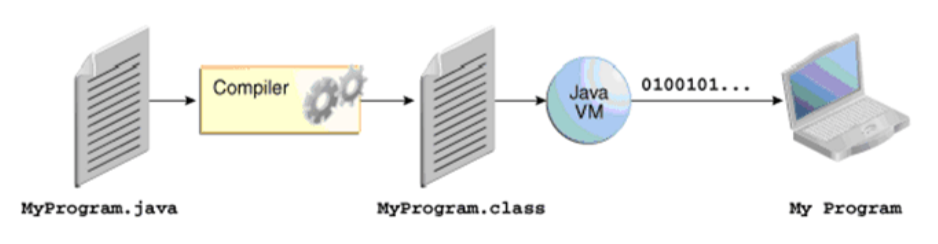
\includegraphics[width=0.7\textwidth]{Img/jvm-architecture.png}
    \caption{Java architecture}
    \label{JavaArchitecture}
\end{figure}

L'architettura del linguaggio Java \`e mostrata in Figura~\ref{JavaArchitecture}. Pi\`u precisamente,

\begin{itemize}
\item MyProgram.java: \`e il codice sorgente nativo dell'applicazione Java (Il file che contiene il nostro codice)
\item Compiler: (Compilatore) prende in input il nostro codice Java  (i nostri files \texttt{.java}), e produce dei file intermedi  (\texttt{.class}) ovvero i file contenenti il byte-code.
\item Java Virtual Machine: \`e l'interprete che deve essere installato sulla nostra macchina locale al fine di eseguire il byte-code. Il byte-code viene interpretato dalla Java Virtual Machine. Per questo motivo alcuni testi considerano Java anche come un linguaggio interpretato.
\end{itemize}

Per eseguire il vostro programma su una macchina \`e sufficiente che l'utente abbia installato una macchina virtuale: Java Virtual Machine. In particolare, il Java Run-time Environment (JRE) contiene la macchina virtuale che consente di eseguire i programmi Java.  JREs differenti sono associati a sistemi operativi differenti. Tuttavia, una volta generati, i class files possono essere eseguiti su ogni sistema cha abbia una Macchina Virtuale installata. \\
Per compilare i tuoi file Java \`e necessario avere un tool di sviluppo Java: un Java Development Kit (JDK). Il JDK include la JRE e contiene un set di tool di svilupo che constentono di scrivere e compilare i tuoi programmi Java.




\subsubsection{Java is object oriented}
In an object oriented programming language the main building block of a program is an object.
\begin{mydef} (Object) A Java \texttt{object} is an abstraction of a real word object, and  describes the characteristics of the real word object that are of interest for the developer.
\end{mydef}
In this paradigm the developer describes the \emph{the word} (the objects of the word) and how \emph{the word can change over time} (the states can change over time). This paradigm is different from procedural modeling languages where the main building block is the procedure which modifies the value of a program. In procedural modeling languages the developer specifies \emph{how to solve} a problem, while in object oriented modeling language the developer first describes the \emph{world} and \emph{how it is possible to change the world} and then find a strategy to solve the problem giving the model previously constructed. In other words, differently from languages such as $C$ in which first you think about function and then on the structure of the manipulated data, in $Java$ and in general in an object oriented language you \emph{first think on the data and modeling the problem} and then how the to change these data. 

\begin{lstlisting}
new Bike();
\end{lstlisting}
Every object is instantiated (created) with the instruction \emph{new} and is described though a class. For example, the previous instruction creates a new object of class \texttt{Bike}.

\begin{mydef} (Class) A \texttt{class} is a \emph{type} defined by the user that describes an object. More precisely it describes how the state of the system can be identified and how the state can change in response with operations that can be executed over this object.
\end{mydef}

In Java a class is a description of the object of the real word and is a blueprint for the generation of the objects that can be created (instantiated) into the system. 

\begin{lstlisting}[language=Java,escapechar=|]
public class Bike {

	public Bike(){
	}
}
\end{lstlisting}
Class are defined through the keyword \texttt{class} and describe how the state of an object is identified and how this state can change.

Finally, Java is statically typed.
\begin{mydef} (Statically typed) A language is \emph{statically typed} if every variable name is associated both
to a type and to an object.
\end{mydef}
\begin{lstlisting}
Bike bike1=new Bike();
\end{lstlisting}
For example, the previous instruction declares a variable \texttt{bike1} which \emph{has} type \texttt{Bike} and is associated to an object of class \texttt{Bike}. Since each variable must be associated to a type the language is statically typed.

\section{Exercises}
\begin{itemize}
\item The goal of the first exercise is to show the main advantage of using Java and, more precisely how java supports portability.
\item Let's crate our first Java project
\end{itemize}

\subsubsection{Creating a Java File}
\begin{itemize}
\item Open TextEdit (for mac users), Blocco Note (for Windows users) of vi (for Linux) users.
\item (For Mac User from TextEdit choose \textit{preferenze} $>$ \textit{Solo Testo} $>$ \textit{File} $>$ \textit{New} )
\item Type the following Java code
\end{itemize}
\begin{lstlisting}
public class Welcome {	
    public static void main(String[] args){	
	 	System.out.println("Benvenuto al corso di Ingegneria del Software");
    }
}
\end{lstlisting}
\begin{itemize}
\item Save the file as Welcome.java (Note: be sure that another extension is not selected).
\end{itemize}

\subsubsection{Compiling the Java File}
\begin{itemize}
\item open the Terminal (for Mac and Linux users) or the Command Propt (for Windows users)
\item locate the file created - useful commands 
\begin{itemize}
\item for Mac and Linux Users it is possible to open a folder with \emph{cd}, exit from a folder with \emph{cd ..} and show the content of a folder with \emph{ls}) 
\item
\end{itemize}
\item Type \texttt{javac Welcome.java}
\item This command \textbf{compliles} the Welcom.jar file and generates a .class (or a jar) file which contains the a bytecode file that can be executed on the different platforms\footnote{The bytecode is an intermediate representation that can be interpreted by a Virtual Machine.}. This process supports \textbf{portability}.
\item \emph{To run the javac command a JDK (Java Development Kit) must be installed in your pc\footnote{The JDK also include the Java Run-Time Environment which will be later introduced}.} The JDK allows to \emph{compile} and \emph{execute} the created programs and several \emph{libraries} which are commonly used in the development.
\end{itemize}

\subsubsection{Running the Java File}
\begin{itemize}
\item the java bytecode file (.class) can be executed on each architecture over which a Virtual Machine (which provides an \textbf{interpreter} for the $Java$ bytecode) for Java is installed. The Java JRE provides this Virtual Machine.
\item to run the java bytecodefile run type \texttt{java Welcome}
\item the command java Welcome executes the \texttt{Main} method of the class Welcome
\end{itemize}

\subsubsection{Our first Java program}
\begin{lstlisting}
public class Welcome {	
    public static void main(String[] args){	
	 	System.out.println("Benvenuto al corso di Ingegneria del Software");
    }
}
\end{lstlisting}
\begin{itemize}
\item The code specified defines a \texttt{class} called Welcome with a single \texttt{method} called main
\item \texttt{public} is used to specify that the class and the corresponding method can be accessed by an external client (such as other classes).
\item \texttt{class} is used to specify a new type of data
\item \texttt{void} specifies that the method does not return any value
\item \texttt{static} specifies that the method can be invoked without creating the corresponding object (Welcome)
\item \texttt{main} is a ``starting method" that \textbf{must} be present in at least one class for the application to be run.
\item \texttt{args} contains the parameter of the main argument. The parameters (also called arguments) are variables that can contains values that are passed to the method when is called. The parameters must have a type
\item \texttt{String[]} (array of String) is the type of the args parameter 
\item the arg parameter is used from main to obtain arguments that can be passed when the method is invoked from command line
\item \texttt{System.out.println} writes the specified text on the screen
\end{itemize}

\subsubsection{Our second Java program}
Change the previously described program to:
\begin{itemize}
\item to require the user to insert is name (for example Carlo)
\item to print ``Ciao Carlo, Benvenuto al corso di Ingegneria del Software" 
\end{itemize}
Solution:
\begin{itemize}
\item create a new Java file with name \texttt{WelcomeWithName}
\item type the following
\end{itemize}
\begin{lstlisting}[
    language=Java,escapechar=|]
import java.util.Scanner;

public class WelcomeWithName {
	public static void main(String[] args){
		Scanner scanner = new Scanner(System.in); |\label{line:scanner}|
		System.out.println("Inserisci il tuo nome:");
		String nome = scanner.nextLine();
		scanner.close();
		String welcome = "Benvenuto al corso di Ingegneria del Software";
		System.out.println("Ciao " + nome + ", " + welcome);
	}
}
\end{lstlisting}
\begin{itemize}
\item \texttt{import} is used to import the \texttt{class} Scanner which is contained in the \texttt{java.util} package
\item \texttt{new} creates (\texttt{instantiate}) a new Scanner Object
\item \texttt{scanner.nextLine()} reads the next of the current line
\item \texttt{scanner.close()} close the scanner
\end{itemize}


\subsection{Object-orientated (30 min)}
\textbf{Problem}
\begin{itemize}
\item Try to model a Bike
\end{itemize}

To design your Bike you (or the client) must answer two main questions:
\begin{itemize}
\item How can you define the \textbf{state} of the bike?
\item Which \textbf{functionalities} offers the bike?
\end{itemize}


\subsubsection{Modeling a Bike 1}
\begin{itemize}
\item Let's start considering the \textbf{state} of the bike
\end{itemize}
A bike has a certain SPEED that depends on the GEAR (marcia) and on the CADENCE (ritmo di pedalata).

\begin{lstlisting}[language=Java,escapechar=|]
// defines a public class called Bike 
// the name of the class usually starts with an upper case letter
public class Bike {
	
	// The attributes of the class are used to describe the state of the class and are usually private or protected 
	// The attributes of the class usually start with lower case letters
	private int gear=1; //default 1
	private int cadence; //default 0
	private int speed; //default 0
	
	// is the constructor of the class which allows to create a new Bike
	// the constructor has the same name of the class and does not have a return type
	public Bike(){
	}
}
\end{lstlisting}

\textbf{Implementing a client}
\begin{itemize}
\item A client (generally) is a generic user of classes (e.g., a class provided of a Main method).
\end{itemize}

\begin{lstlisting}[language=Java,escapechar=|]
public class Client {
	
	public static void main(String[] args)
    {
        Bike bike1; // defines a new reference (pointer) of class Bike with a predefined value null
        bike1 = new Bike(); // instantiate  the object
        // the instruction new Bike() creates a new object of type Bike and returns the reference to this object which is assigned to the reference bike1
        // when the method new is invoked, the VM allocates dynamically the quantity of memory which is sufficient to contain the Bike object
        Bike bike2 = new Bike(); // defines and instantiate a new object of class Bike
     }
}
\end{lstlisting}
To run the program compile the Bike and the Client and run the Client

\textbf{Questions?}\\
\begin{itemize}
\item Which is the state of the object after the instruction \emph{Bike bike1;}? the object does not exists it only exists the corresponding reference.
\item Which is the state of the object \texttt{bike1} after the instruction \texttt{bike1 = new Bike();}? \texttt{gear=1}, \texttt{cadence=0}, \texttt{speed=0}
\item Which is the state of the object \texttt{bike1} after the instruction \texttt{bike2 = new Bike();}? \texttt{gear=1}, \texttt{cadence=0}, \texttt{speed=0}
\item Which is the state of the object \texttt{bike2} after the instruction \texttt{bike2 = new Bike();}? \texttt{gear=1}, \texttt{cadence=0}, \texttt{speed=0}
\end{itemize}



\subsubsection{Modeling a Bike 2}
\begin{lstlisting}[language=Java,escapechar=|]
public class Client {
	
	public static void main(String[] args)
    {
        Bike bike1; 
        bike1 = new Bike();
        Bike bike2 = new Bike(); 
        
        // == compare the reference of the Bike1 with the reference of the Bike2
        System.out.println(bike1==bike2);
     }
}
\end{lstlisting}

\textbf{Questions?}\\
\begin{itemize}
\item What does the instruction \texttt{bike1==bike2} print? false, since the two references \texttt{bike1} and \texttt{bike2} refers to different objects
\end{itemize}

\subsubsection{Modeling a Bike 3}
\begin{itemize}
\item Let's start considering the \textbf{functionalities} of the bike
\end{itemize}
The Bike must be able to print its state

\begin{lstlisting}[language=Java,escapechar=|]
// defines a public class called Bike 
// the name of the class usually starts with an upper case letter
public class Bike {
	
	// The attributes of the class are used to describe the state of the class and are usually private or protected 
	// The attributes of the class usually start with lower case letters
	private int gear=1; //default 1
	private int cadence; //default 0
	private int speed; //default 0
	
	// is the constructor of the class which allows to create a new Bike
	// the constructor has the same name of the class and does not have a return type
	public Bike(){
	}
	
	public void printState(){
	    // + is the String concatenation operator
	    // the int gear, speed and cadence are automatically converted into String
		System.out.println("gear: "+ gear + ", speed: "+speed+ ", cadence: "+cadence);
	}
}
\end{lstlisting}

\subsubsection{Modeling a Bike 3 - packages}
\begin{lstlisting}[language=Java,escapechar=|]
package transport;

// defines a public class called Bike 
// the name of the class usually starts with an upper case letter
public class Bike {
	
	// The attributes of the class are used to describe the state of the class and are usually private or protected 
	// The attributes of the class usually start with lower case letters
	private int gear=1; //default 1
	private int cadence; //default 0
	private int speed; //default 0
	
	// is the constructor of the class which allows to create a new Bike
	// the constructor has the same name of the class and does not have a return type
	public Bike(){
	}
	
	public void printState(){
	    // + is the String concatenation operator
	    // the int gear, speed and cadence are automatically converted into String
		System.out.println("gear: "+ gear + ", speed: "+speed+ ", cadence: "+cadence);
	}
}
\end{lstlisting}

\begin{lstlisting}[language=Java,escapechar=|]
// imports the class Bike inside the package transport
import transport.Bike;

public class Client {
	
	public static void main(String[] args)
    {
        Bike bike1; 
        bike1 = new Bike();
        Bike bike2 = new Bike(); 
        
        // == compare the reference of the Bike1 with the reference of the Bike2
        System.out.println(bike1==bike2);
        // invokes the method print state of the object bike1       
          bike1.printState();
          // invokes the method print state of the object bike2
            bike2.printState();

     }
}
\end{lstlisting}

If we change folder of the bike class we have to change the package

\subsection{Eclipse Integrated Development Environment  (20 min)}
\begin{itemize}
\item The procedure previously described is tedious and error prone, in particular when the complexity of the project increases, packages are added etc.
\item for this purpose, in the software development,  Integrated Development Environment ($IDE$) are commonly used. $IDE$s remove some of the difficulties usually encountered during the compilation process and provides additional features, such as code completion.
\item In this course we will use the $Eclipse$ $IDE$\footnote{$Netbeans$ one of the most used competitor of $Eclipse$}.  
\end{itemize}

\subsubsection{Creating your first project using Eclipse}
\begin{itemize}
\item double click on $Eclipse$
\item when $Eclipse$ starts it asks the user to specify the $Workspace$. The $Workspace$ is the ``place" over which the user wants to work. The user can define different $Workspace$s each of which can contain \emph{multiple projects}.
\item press on $Workbench$ (banco di lavoro)
\item \texttt{File} $>$ \texttt{New} $>$ \texttt{Project} $>$ \texttt{Maven Project}
\item check \texttt{Create a simple project}
\item type \texttt{IngegneriaDelSoftware1} as Group Id and \texttt{Esercitazione1} as Artifact Id
\item choose \texttt{finish}
\end{itemize}

When you create a new Project (Maven\footnote{Maven will be explained in the lab.}) in Eclipse, it automatically generates a structure for your project. In particular, 
\begin{itemize}
\item $src/main/java$ contains the java source code of the application under development
\item $src/main/resources$ contains the resources used from the application
\item $src/test/java$ contains the classes which are used to test the application under development
\item $src/test/resources$ contains the resources used from the test classes to test the application
\end{itemize}

\subsubsection{Creating a new Package in Eclipse}
To create a new Package in Eclipse
\begin{itemize}
\item right click on \texttt{src/main/java} $>$ New $>$ package 
\item type a name for your class ($esercitatione1$)
\item press finish
\end{itemize}

\subsubsection{Creating a new Class in Eclipse}
To create a new Class in Eclipse
\begin{itemize}
\item right click on the place in which you want to create the new class  (for example the package esercitazione1) $>$ New $>$ class 
\item type a name for your class (\texttt{Bike})
\item choose the visibility of the class etc...
\item press finish
\end{itemize}
As you can see the $IDE$ automatically compiles the package of the class the identifiers, etc (and it is able to do other stuff that will be explained during the course).


\subsubsection{Running a project in Eclipse}
\label{sec:runningAProjectInEclipse}
To run a project in eclipse
\begin{itemize}
\item right click on the class that you want to run (\emph{it must contain a main method})
\item Run As $>$ Java Application
\end{itemize}

\subsubsection{What is going on?}
If you open your workspace and your project you will see two different folders:
\begin{itemize}
\item src: contains the source file of your application (\texttt{.java} files)
\item target: contains the bytecode files (\texttt{.class} files) which are generated when you perform the procedure explained in~\ref{sec:runningAProjectInEclipse} and then are runned.
\end{itemize}

\subsection{Object-oriented 2 (10 min)}

\subsubsection{Modeling a Bike 4}
Add the following functionality
\begin{itemize}
\item it must be possible to monitor the \texttt{gear}, the \texttt{cadence} and the \texttt{speed} of the Bike
\end{itemize}

``Monitoring" is done through getters.\\
Command tricks:
\begin{itemize}
\item Control + Space : allows to automatically complete the text and provides suggestions
\end{itemize}

\begin{lstlisting}[language=Java,escapechar=|]
package esercitatione1;


//defines a public class called Bike 
//the name of the class usually starts with an upper case letter
public class Bike {
	
	// The attributes of the class are used to describe the state of the class and are usually private or protected 
	// The attributes of the class usually start with lower case letters
	private int gear=1; //default 1
	private int cadence; //default 0
	private int speed; //default 0
	
	// is the constructor of the class which allows to create a new Bike
	// the constructor has the same name of the class and does not have a return type
	public Bike(){
	}
	
	public void printState(){
	    // + is the String concatenation operator
	    // the int gear, speed and cadence are automatically converted into String
		System.out.println("gear: "+ gear + ", speed: "+speed+ ", cadence: "+cadence);
	}
	
	// returns the gear of the bike
	public int getGear(){
		return this.gear;
	}

	// returns the cadence of the bike
	public int getCadence(){
		return this.cadence;
	}
	
	// returns the speed ok the bike
	public int getSpeed(){
		return this.speed;
	}
}
\end{lstlisting}


\begin{lstlisting}[language=Java,escapechar=|]
package esercitatione1;

public class Client {

	public static void main(String[] args) {

		Bike bike1;
		bike1 = new Bike();
		Bike bike2 = new Bike();

		// == compare the reference of the Bike1 with the reference of the Bike2
		System.out.println(bike1 == bike2);
		// invokes the method print state of the object bike1
		bike1.printState();
		// invokes the method print state of the object bike2
		bike2.printState();

		System.out.println(bike1.getCadence());
	}

}

\end{lstlisting}


\subsubsection{Modeling a Bike 5}
Add the following functionality
\begin{itemize}
\item increase and decrease the gear and change the cadence and update the speed consequently
\end{itemize}

``Monitoring" is done through getters.\\
Command tricks:
\begin{itemize}
\item Control + Space : allows to automatically complete the text and provides suggestions
\end{itemize}

\begin{lstlisting}[language=Java,escapechar=|]
package esercitatione1;

//defines a public class called Bike 
//the name of the class usually starts with an upper case letter
public class Bike {

	// The attributes of the class are used to describe the state of the class
	// and are usually private or protected
	// The attributes of the class usually start with lower case letters
	private int gear=1; // default 1
	private int cadence; // default 0
	private int speed; // default 0

	// is the constructor of the class which allows to create a new Bike
	// the constructor has the same name of the class and does not have a return
	// type
	public Bike() {
	}

	public void printState() {
		// + is the String concatenation operator
		// the int gear, speed and cadence are automatically converted into
		// String
		System.out.println("gear: " + gear + ", speed: " + speed
				+ ", cadence: " + cadence);
	}
    
    // changes the cadence of the bike
	public void changeCadence(int cadence) {
		this.cadence = cadence;
		updateSpeed();
	}

	// increment the gear
	public void incrementGear() {
		this.gear++;
		this.updateSpeed();
	}

	// decrement the gear
	public void decrementGear() {
		this.gear--;
		this.updateSpeed();
	}

	// every time the cadence or the gear changes the speed is updated
	// the method is private and cannot be invoked from other external classes
	private void updateSpeed(){
		this.speed = this.gear * this.cadence; 
	}
	
	// returns the gear of the bike
	public int getGear() {
		return this.gear;
	}

	// returns the cadence of the bike
	public int getCadence() {
		return this.cadence;
	}

	// returns the speed ok the bike
	public int getSpeed() {
		return this.speed;
	}
}
\end{lstlisting}


\begin{lstlisting}[language=Java,escapechar=|]
package esercitatione1;

public class Client {

	public static void main(String[] args) {

		Bike bike1;
		bike1 = new Bike();
		Bike bike2 = new Bike();

		// == compare the reference of the Bike1 with the reference of the Bike2
		System.out.println(bike1 == bike2);
		// invokes the method print state of the object bike1
		bike1.printState();
		// invokes the method print state of the object bike2
		bike2.printState();

		bike1.printState();
		bike1.incrementGear();
		bike1.printState();
		
		bike1.changeCadence(10);
		bike1.printState();
		
	}
}
\end{lstlisting}

\textbf{Questions?}\\
\begin{itemize}
\item What is  the state of the object \texttt{bike1} after the instruction  \texttt{bike1.incrementGear();} is performed? 
\texttt{gear=2}, \texttt{cadence=0}, \texttt{speed=0}.
\item What is  the state of the object \texttt{bike1} after the instruction  \texttt{bike1.changeCadence(10);} is performed? 
\texttt{gear=2}, \texttt{cadence=10}, \texttt{speed=0}.
\end{itemize}

\subsubsection{Modeling a Bike 6}
\begin{itemize}
\item the gears of the type of Bike that is considered are $6$ 
\end{itemize}

\begin{lstlisting}[language=Java,escapechar=|]
package esercitatione1;

//defines a public class called Bike 
//the name of the class usually starts with an upper case letter
public class Bike {

	// static specifies that this variable is shared from all the objects
	// The final modifier indicates that the value of this field cannot change.
 	// The static modifier, in combination with the final modifier, is also used to define constants. 
	private static final int MAX_GEAR = 6;
	private static final int MIN_GEAR = 1;

	// The attributes of the class are used to describe the state of the class
	// and are usually private or protected
	// The attributes of the class usually start with lower case letters
	private int gear = 1; // default 1
	private int cadence; // default 0
	private int speed; // default 0

	// is the constructor of the class which allows to create a new Bike
	// the constructor has the same name of the class and does not have a return
	// type
	public Bike() {
	}

	public void printState() {
		// + is the String concatenation operator
		// the int gear, speed and cadence are automatically converted into
		// String
		System.out.println("gear: " + gear + ", speed: " + speed
				+ ", cadence: " + cadence);
	}

	// changes the cadence of the bike
	public void changeCadence(int cadence) {
		this.cadence = cadence;
		updateSpeed();
	}

	// increment the gear
	public void incrementGear() {
		if (gear < MAX_GEAR) {
			gear++;
			updateSpeed();
		}
	}

	// decrement the gear
	public void decrementGear() {
		if (gear > MIN_GEAR) {
			gear--;
			updateSpeed();
		}
	}

	// every time the cadence or the gear changes the speed is updated
	// the method is private and cannot be invoked from other external classes
	private void updateSpeed() {
		this.speed = this.gear * this.cadence;
	}

	// returns the gear of the bike
	public int getGear() {
		return this.gear;
	}

	// returns the cadence of the bike
	public int getCadence() {
		return this.cadence;
	}

	// returns the speed ok the bike
	public int getSpeed() {
		return this.speed;
	}
}
\end{lstlisting}


\subsubsection{Modeling a Bike 7}
\begin{itemize}
\item change the Bike class in a way that it is possible to create a Bike with a specified gear and cadence
\end{itemize}

\begin{lstlisting}[language=Java,escapechar=|]
package esercitatione1;

//defines a public class called Bike 
//the name of the class usually starts with an upper case letter
public class Bike {

	// static specifies that this variable is shared from all the objects
	// The final modifier indicates that the value of this field cannot change.
 	// The static modifier, in combination with the final modifier, is also used to define constants. 
	private static final int MAX_GEAR = 6;
	private static final int MIN_GEAR = 1;

	// The attributes of the class are used to describe the state of the class
	// and are usually private or protected
	// The attributes of the class usually start with lower case letters
	private int gear = 1; // default 1
	private int cadence; // default 0
	private int speed; // default 0

	// is the constructor of the class which allows to create a new Bike
	// the constructor has the same name of the class and does not have a return
	// type
	// gear and cadence are the intial values of the gear and the cadence
	public Bike(int gear, int cadence) {
		
		// this allows to refer to the variable gear of THIS class, otherwise gear refers to the variable passed as parameter
		this.gear=gear;
		this.cadence=cadence;
		this.updateSpeed();
	}

	public void printState() {
		// + is the String concatenation operator
		// the int gear, speed and cadence are automatically converted into
		// String
		System.out.println("gear: " + gear + ", speed: " + speed
				+ ", cadence: " + cadence);
	}

	// changes the cadence of the bike
	public void changeCadence(int cadence) {
		this.cadence = cadence;
		updateSpeed();
	}

	// increment the gear
	public void incrementGear() {
		if (gear < MAX_GEAR) {
			gear++;
			updateSpeed();
		}
	}

	// decrement the gear
	public void decrementGear() {
		if (gear > MIN_GEAR) {
			gear--;
			updateSpeed();
		}
	}

	// every time the cadence or the gear changes the speed is updated
	// the method is private and cannot be invoked from other external classes
	private void updateSpeed() {
		this.speed = this.gear * this.cadence;
	}

	// returns the gear of the bike
	public int getGear() {
		return this.gear;
	}

	// returns the cadence of the bike
	public int getCadence() {
		return this.cadence;
	}

	// returns the speed ok the bike
	public int getSpeed() {
		return this.speed;
	}
}
\end{lstlisting}

\begin{lstlisting}[language=Java,escapechar=|]
package esercitatione1;

public class Client {

	public static void main(String[] args) {

		Bike bike1;
		bike1 = new Bike(3, 2);
		Bike bike2 = new Bike(1, 2);

		// == compare the reference of the Bike1 with the reference of the Bike2
		System.out.println(bike1 == bike2);
		// invokes the method print state of the object bike1
		bike1.printState();
		// invokes the method print state of the object bike2
		bike2.printState();

		bike1.printState();
		bike1.incrementGear();
		bike1.printState();
		bike1.changeCadence(10);
		bike1.printState();
	    }
}
\end{lstlisting}
\textbf{Questions?}\\
\begin{itemize}
\item What is  the state of the object \texttt{bike1} after the instruction  \texttt{bike1=new Bike(3, 2);} is performed? 
\texttt{gear=3}, \texttt{cadence=2}, \texttt{speed=0}.
\item What is  the state of the object \texttt{bike2} after the instruction  \texttt{Bike bike2=new Bike(1, 2);} is performed? 
\texttt{gear=1}, \texttt{cadence=2}, \texttt{speed=0}.
\item What is  the state of the object \texttt{bike1} after the instruction  \texttt{bike1.incrementGear();} is performed? 
\texttt{gear=3}, \texttt{cadence=2}, \texttt{speed=0}.
\item What is  the state of the object \texttt{bike1} after the instruction  \texttt{bike1.changeCadence(10);} is performed? 
\texttt{gear=3}, \texttt{cadence=10}, \texttt{speed=0}.
\end{itemize}

\section{Curiosity}
\begin{framed}
The name Java reflected the teams’ love for coffee. Indeed, Java coffee refers to coffee beans produced in the Indonesian island of Java.
\end{framed}

\clearpage

% ---- Bibliography ----




\addcontentsline{toc}{chapter}{Bibliography}
\bibliographystyle{alpha}
\bibliography{Intro}
\nocite{*}


\end{document}

